
\chapter{Related work: Multi-agent formalisms}
\label{chap:related}
%\section{Aims}
%\label{sec:marl}
Multi-agent learning (MAL) problems are problems where an agent is to learn to behave optimally in the company of other agents, which may or may not be learning themselves \cite{Tuyls_Weiss_2012}.
Multi-agent settings are inherently more complex than their single-agent counterpart. In particular, several useful properties that hold in single-agent settings are no longer valid in multi-agent settings. Nevertheless, MAL techniques are used in practice and generally produce good results \cite{fundamentallymoredifficult}. \RefSec{sec:additional} addresses some of the challenges that arise when moving from a single-agent setting to a multi-agent setting. Sections \ref{sec:mmdp}, \ref{sec:decpomdp}, and \ref{sec:ipomdp} then summarize several multi-agent frameworks. Finally, \RefSec{sec:repnet} covers the multi-agent, POMDP-based framework called \textit{Reputation Network} POMDP.
\section{Challenges in multi-agent formalisms}
\label{sec:additional}
\subsection{Non-stationarity}
An intuitive and naive way of dealing with the presence of multiple agents from the perspective of one agent $g$ may be to consider every other agent to be a part of the environment. In fact, by assuming that each agent $h$ is following a stationary policy $\pi_h$, solving a MAL problem from the perspective of agent $g$ reduces to solving a single-agent problem where the behavior of all other agents is factored in the environment's transition model \cite{reduce, reduce2}. This assumption is not always reasonable and, more often than not, the agents will adapt their policy as time goes by \cite{nonstation}. Alongside the impossibility of reducing the problem, \textit{correlated goals} and the \textit{loss of convergence guarantee} discussed hereafter have a significant impact on multi-agent learning.

\subsection{Correlated goals}
In single-agent settings, the rewards collected by the agent are a function of the state of the environment. In multi-agent settings, a first consequence of the non-stationarity of policies is that one agent's returns will likely depend on the other agents' behavior as well \cite{nonstation}. Explicit modeling of the reward scheme may, therefore, be significantly more complex.

\subsection{The convergence problem}
Another consequence of the non-stationarity of policies is the invalidation of the convergence guarantee of most Single-agent learning (SAL) algorithms \cite{nonstation, convergence}. In fact, the convergence of one agent's policy is now a function of all other agents' behavior in the network.

\subsection{The curse of dimensionality}
In complexity theory, a problem is considered to suffer from the curse of dimensionality with respect to a variable $n$ if
\begin{align}
    \label{eq:intract}
    T(n) = \Omega(2^n),
\end{align}
where $\Omega$ is the lower-bound on complexity, and $T$ is the number of steps required to solve said problem \cite{cursedim2}. Such a problem is said to be \textit{intractable}. Multi-agent learning problems are not the only ones subject to the curse of dimensionality: in fact, \RefSec{sec:intract} already illustrated the intractability of solving classic single-agent POMDPs via \textit{Value Iteration}. The problem worsens considerably when moving to multi-agent frameworks \cite{cursedim}.


\section{Multi-agent MDP: A centralized framework}
\label{sec:mmdp}
The Multi-agent MDP (MMDP) was formalized by Boutilier in 1996 \cite{Boutilier}, and is one of the first and simplest multi-agent learning frameworks.
\begin{definition}[Multi-agent MDP]
\label{def:mmdp}
A multi-agent Markov Decision Process, or simply MMDP, $\mathcal{M}$ is formally defined as a tuple
\begin{align*}
    \mathcal{M} := \big \langle \mathcal{S}, \mathcal{G}, \mathcal{A} = \times_{g \in \mathcal{G}} \mathcal{A}_g, \mathcal{T}, \mathcal{R} \big \rangle
  \end{align*}
where:
\begin{itemize}
    \item $\mathcal{S}$ is the set of possible states of the environment.
    \item $\mathcal{G}$ is the set of agents that can interact with the environment.
    \item $\mathcal{A}_g$ is the set of actions available to agent $g$.
    \item $\mathcal{A}$ is the set of joint actions.
    \item $\mathcal{T} : \mathcal{S} \times \mathcal{A}_1 \times ... \times \mathcal{A}_n \times  \mathcal{S} \rightarrow [0,1]$ is called the \textit{transition model}. 
    \item $\mathcal{R}: \mathcal{S} \times \mathcal{A}_1 \times ... \times \mathcal{A}_n \rightarrow \R$ is called the \textit{team reward function}.
\end{itemize}
\end{definition}



MMDP agents are assumed to be \textit{fully cooperative} \cite{Boutilier}, that is, they have no individual motivation. Their sole goal lies in maximizing the global (i.e. shared) expected reward. Each agent is furthermore assumed to have \textit{individual full state observability}, meaning all agents observe the same state. One can, therefore, think of an MMDP as a \textit{joint-action} MDP in which a single, \textit{central} unit applies \textit{joint actions} to the environment \cite{oliehoek}. The \textit{joint-action} policy 
\begin{align}
    \pi : \mathcal{S} \rightarrow \mathcal{A},
\end{align}
associated with the shared value function $V^{\pi}$ is hereby to be maximized. Having a \textit{central} unit follow the present \textit{joint-action} policy is equivalent to having each agent $g$ follow their respective individual policy $\pi_g : \mathcal{S} \rightarrow \mathcal{A}_g$, derived from $\pi$ \cite{oliehoek}. As such, MMDPs are said to make up a \textit{centralized} framework.



\section{Decentralized-POMDP: Decentralized policy execution}
\label{sec:decpomdp}
A major assumption of MMDPs is that each agent is fully aware of the complete state of the environment, at all times. This assumption may not always be realistic \cite{decmdp}. In 2002, still in the realm of \textit{cooperative} planning, Bernstein et al. \cite{decmdp2} took a \textit{decentralized} approach to MDPs in multi-agent settings, by incorporating the idea of \textit{individual- or local- observations}, as well as having the agents be unaware of the other agents' \textit{observations}. This decentralization is fundamentally different to MMDPs and makes DEC-POMDPs more difficult to solve. It should be noted that, while the \textit{online} phase, i.e. execution of the learned plan, is, in fact, completely decentralized, the \textit{offline} phase, i.e., the actual planning, is centralized \cite{moredec}. More specifically, a single centralized unit computes the joint-action policy offline and then distributes the individual policies to be executed by the agents online.

\begin{definition}[DEC-POMDP]
\label{def:decpomdp}
A decentralized Partially Observable Markov Decision Process, or DEC-POMDP, $\mathcal{D}$ is formally defined as a tuple
\begin{align*}
    \mathcal{D} := \big \langle \mathcal{S}, \mathcal{G}, \mathcal{A} = \times_{g \in \mathcal{G}} \mathcal{A}_g, \Omega = \times_{g \in \mathcal{G}} \Omega_g, \mathcal{T}, \mathcal{R}, \mathcal{O} \big \rangle
  \end{align*}
where:
\begin{itemize}
    \item $\mathcal{S}$, $\mathcal{G}$, $\mathcal{A}_g$, $\mathcal{A}$, $\mathcal{T}$, and $\mathcal{R}$ are defined as in \RefDef{def:mmdp}.
    \item $\Omega_g$ is the set of observations available to agent $g$.
    \item $\Omega$ is the set of joint observations.
    \item $\mathcal{O} : \mathcal{A} \times \mathcal{S} \times \Omega \rightarrow [0,1]$ is called the \textit{joint observation function}.
\end{itemize}
\end{definition}
DEC-POMDPs can be reduced to DEC-MDPs if there exists a mapping $J$ such that
\begin{align}
    J: \Omega_1 \times ... \times \Omega_n \rightarrow S,
\end{align}
in other words, if the joint observation of all agents uniquely identifies the state of the environment. The state is then said to be \textit{jointly fully observable}. It is worth noting that even then, the agents themselves are only aware of their \textit{individual observations} \cite{oliehoek}.

\section{Interactive-POMDP: A framework for self-interested agents}
\label{sec:ipomdp}
In 2005, Gmytrasiewicz et al. formalized a further extension of POMDPs to multi-agent settings, called Interactive-POMDP \cite{ipomdp}. In contrast to MMDPs and DEC-POMDPs, I-POMDPs make no assumption about the willingness of the agents to be \textit{cooperative}. In fact, I-POMDPs are mainly applied to domains made up of \textit{autonomous} and \textit{self-interested} agents. While in DEC-POMDPs the optimal joint policy is computed by a \textit{centralized} unit before being distributed amid the agents, the self-interested nature of I-POMDP agents requires the \textit{learning} algorithms to be \textit{decentralized}, that is, each agent is to locally compute its own policy as a function of its beliefs about the physical state of the environment as well as its interactions with the other agents.

\begin{definition}[I-POMDP]
\label{def:decpomdp}
An Interactive Partially Observable Markov Decision Process, or I-POMDP, of an agent, say $g$, is written $\mathcal{I}_g$ and is formally defined as a tuple
\begin{align*}
    \mathcal{I}_g := \big \langle \mathcal{IS}_g, \mathcal{A} = \times_{g \in \mathcal{G}} \mathcal{A}_g, \Omega_g, \mathcal{T}_g, \mathcal{R}_g, \mathcal{O}_g \big \rangle
  \end{align*}
where:
\begin{itemize}
    \item $\mathcal{IS}_g : \mathcal{S} \times_{h:h \neq g} \mathcal{M}_h$ is the set of interactive states of agent $g$. Interactive states are physical environment states augmented with models of each agent in the network.
    \item $\mathcal{A}_g$ and $\mathcal{A}$ are defined as in \RefDef{def:mmdp}.
    \item $\Omega_g$ is the set of observations available to agent $g$.
    \item $\mathcal{T}_g : \mathcal{S} \times \mathcal{A} \times \mathcal{S} \rightarrow [0,1]$
    \item $\mathcal{R}_g : \mathcal{IS}_g \times \mathcal{A} \rightarrow \R$ is called the \textit{immediate} reward of agent $g$.
    \item $\mathcal{O}_g : \mathcal{A} \times \mathcal{S} \times \Omega_g \rightarrow [0,1]$ is called the \textit{observation function} of agent $g$.
\end{itemize}
\end{definition}
In accordance with the definition of \textit{interactive states}, I-POMDP agents update their beliefs not only over physical states of the environment but also over models of the other agents in the network. The difficulty of solving I-POMDPs lies in the recursive nature of the models. Consider agent $g$'s belief update in a network inhabited by another agent, say $h$. A model of agent $h$ may consist of the belief function of said agent $h$ over physical states and models of all other agents. These models may, in turn, consist of belief functions of their own. This nesting of beliefs could theoretically be infinite, rendering the belief update \textit{non-computable}. This inconvenience is overcome by bounding the nesting depth by a finite number $n$. The problem is then solved as a set of POMDPs. 

In 2009, \textit{Doshi et al.} \cite{monteipomdp} mitigate the computational requirements for solving I-POMDPs by using \textit{Monte Carlo Sampling Methods} to find approximate solutions. In 2011, the complexity of real-world \textit{interactive state spaces} is addressed; \textit{Panella et al.} \cite{impomdprel} introduce a new representation for \textit{interactive states} that draws from \textit{relational} (\textit{first-order}) logic and probability theory, in an attempt to compactly and finitely represent \textit{interactive state spaces}. Recently, in 2019, \textit{Han et al.} \cite{impomdpnn} introduce IPOMDP-Net, a framework that combines I-POMDPs and \textit{Deep Learning}. Their approach is shown to outperform \textit{state-of-the-art} model-free networks. Concretely, IPOMDP-Net is a \textit{deep neural network} that embeds an I-POMDP and a QMDP planner (\cite{qmdp}) in its network architecture.
\section{The RepNet-POMDP framework}
\label{sec:repnet}
This section introduces the multi-agent, POMDP-based framework called Reputation Network POMDP, which was proposed by \textit{Rens et al.} in their paper "\textit{Maximizing Expected Impact in an Agent
Reputation Network}" published in 2018 \cite{rensetal} and constitutes the foundation of the work presented in the rest of the thesis. Several multi-agent frameworks have been presented in this chapter. 

To highlight their differences from the RepNet framework, their domains of use are briefly revised here. MMDPs and DEC-POMDPs serve a similar purpose in that they are used to compute a global policy that maximizes the collective well-being of the agents that make up the framework. Consequently, said agents are assumed to be completely selfless. This heavily contrasts with the intended purpose of the RepNet framework, in which each agent uses its \textit{own} instance of the framework, and in which no assumption is made concerning their selflessness. I-POMDPs do serve a similar purpose as far as not making assumptions about an agent's selflessness. They are, however, arguably significantly more difficult to conceptualize than the framework presented hereafter. The RepNet framework achieves a more intuitive layout by making assumptions about the elements that should matter to the agents. In particular, agent \textit{reputation} and \textit{past behavior} of agents are key drivers of the interactions between the agents of the network.


The working principles of the framework are first introduced, after which its planning algorithm is detailed. Note that this section summarizes the framework in its entirety: a few concepts presented hereafter play a minor role in the remainder of this thesis. More concretely, the concepts of \textit{partial observability} and \textit{state estimation} will be worked out of the framework in \RefChap{chap:mdp}. The most important concepts of the framework will be reiterated when necessary in future chapters. 


\subsection{Presentation of the framework}
The \textit{RepNet} framework is aimed at solving multi-agent learning problems in which each agent is associated with a reputation in the network, and their reputation, as well as past behavior, dictate the willingness of the rest of the network to engage in communications with them. Similarly to classic POMDP systems, the rules of \textit{stochasticity} and \textit{partial observability} apply to the environments considered here.
Intuitively, the framework can be thought of as the combinations of 4 pillars.

    \paragraph{The underlying Markov Decision Process structure:} RepNet agents move about in a \textit{stochastic} environment characterized by a set of \textit{states}, and the rules of the environment are described in a \textit{transition model}. RepNet agents progress in the environment by applying one of the \textit{actions} at their disposal. The primary goal of RepNet agents is the \textit{maximization of its long-term cumulative reward}.
    
    \paragraph{A tracking mechanism of other agents' past behavior:} The actions taken by a RepNet agent are informed at all times by the past behavior of other agents in the network.
    
    \paragraph{A tracking mechanism of other agents' reputation:} Each agent has an opinion, be it good or bad, of the remaining agents in the network. RepNet agents explicitly monitor the image they \textit{believe} all agents to have of one another, and use this information in their decision-making process.
    
    \paragraph{A tracking mechanism of the environment's current potential states:} Analogously to Partially Observable Markov Decision Processes, RepNet agents are uncertain of the current state of the environment. Additionally, said agents monitor the state of the environment other agents believe to be in. 


\paragraph*{}The formal presentation of the framework follows hereafter.

\begin{definition}[RepNet-POMDP]\label{def:name}
Let $\Sigma$ be a tuple embedding global information about the system, i.e. the environment and agents that are part of said system, and $\Gamma$ be a tuple embedding each agent's subjective understanding of the environment it operates in. 
A \textit{reputation network POMDP} $\mathcal{M}$ is formally defined as a tuple
  \begin{align*}
    \mathcal{M} := \big \langle \Sigma, \Gamma \big \rangle.
  \end{align*}

\end{definition}

\begin{definition}[System]
\label{def:systempo}
A system $\Sigma$ is formally defined as a tuple
\begin{align*}
    \Sigma := \big \langle \mathcal{G}, \mathcal{S}, \mathcal{A}, \Omega, \mathcal{I}, \mathcal{U} \big \rangle
  \end{align*}
where:
\begin{itemize}
    \item $\mathcal{G}$ is the set of agents that can interact with the environment.
    \item $\mathcal{S}$ is the set of possible states of the environment.
    \item $\mathcal{A}$ is the set of possible actions, both \textit{directed} towards a particular agent and \textit{undirected}. Formally,
    \begin{align*}
    \mathcal{A} := \mathcal{A}^d \cup \mathcal{A}^u\\
    \mathcal{A}^d \cap \mathcal{A}^u := \varnothing
  \end{align*}
  Note that the concept of \textit{undirected actions} is identical to the concept of actions in classic MDPs. The concept of \textit{directed actions} will be discussed in greater detail in \RefSec{sec:dirr}.
  
  \item $\Omega$ is the set of observations.
  \item $\mathcal{I}: \mathcal{G} \times \mathcal{G} \times \mathcal{S} \times \mathcal{A} \rightarrow [-1,1]$ is called the \textit{impact function}. $\mathcal{I}(g,h,s,a)$ returns the impact on agent $g$ that is due to agent $h$ performing action $a$ in state $s$. This function can be thought of as analogous to a Markov Decision Process's immediate reward function $\mathcal{R}$.
  \item $\mathcal{U} : [0,1] \times [-1,1] \times [-1,1] \rightarrow [-1,1]$ is called the \textit{image update function}. Given a learning rate $\alpha$, a current value $v$, of the image on agent has of another agent, to be updated, and a new expected total impact $i$, of which the definition will be given shortly, $\mathcal{U}(\alpha, v, i)$ returns an updated value of the image $v'$.
\end{itemize}
\end{definition}


\begin{definition}[Agents]
\label{def:agentspo}
Let $\Gamma$ be a tuple embedding each agent's subjective understanding of the environment it operates in, such that
\begin{align*}
    \Gamma := \big \langle \{UT_g\}, \{DT_g\},\{O_g\}, \{AD_g\}, \{Img_g\}, \{B_g\} \big \rangle
  \end{align*}
where:
\begin{itemize}
    \item $UT_g : \mathcal{G} \times \mathcal{S} \times \mathcal{A}^u \times \mathcal{S} \rightarrow [0,1]$ is called the \textit{undirected transition model} of agent $g$. $UT_g(h,s,a,s')$ returns the probability of the environment transitioning from state $s$ to state $s'$ when undirected action $a$ is taken by agent $h$.
    \item $DT_g : \mathcal{G} \times \mathcal{S} \times \mathcal{A}^d \times \mathcal{S} \times [-1,1] \rightarrow [0,1]$ is called the \textit{directed transition model} of agent $g$. $DT_g(h,s,a_{h\rightarrow i},r_h,s')$ returns the probability of the environment transitioning from state $s$ to state $s'$ when agent $h$ performs directed action $a_{h\rightarrow i}$ towards another agent, say $i$, and has a reputation $r_h$ according to agent $g$.
    
    \item $O_g$ is called the \textit{observation function}, or \textit{sensor model}, of agent $g$. $O_g(h,a,s',o)$ returns the probability of agent $g$ making observation $o$ after agent $h$, which may or may not be the same as $g$, performs action $a$ and the environment transitions to state $s'$.
    \item $AD_g : \mathcal{G} \times \mathcal{S} \rightarrow \Delta(\mathcal{A})$ is called the \textit{action distribution} of agent $g$. $AD_g(h,s)$ returns a probability distribution over actions in $\mathcal{A}$ for agent $h$ in state $s$, according to agent $g$.
    \item $Img_g : \mathcal{G} \times \mathcal{G} \rightarrow [-1,1]$ is called the \textit{image function} of agent $g$. $Img_g(h,i)$ returns the image agent $i$ has of agent $h$ according to agent $g$.
    \item $B_g : \mathcal{G} \rightarrow \Delta(\mathcal{S})$ is called the \textit{belief state} of agent $g$. $B_g(h)$ (generally written $b_h^g$ hereafter to simplify the notation) returns the belief state of agent $h$, according to agent $g$.
\end{itemize}
\end{definition}
The image two agents have of each other is conditioned by the \textit{impact} they are expected to have on each other, given their current understanding of the state the environment is in. The notion of expected total impact is formalized in \RefDef{def:imppo}, while its effect on the image function is defined in \RefDef{def:imgb}.
\begin{definition}[Expected total impact]
\label{def:imppo}
According to agent $g$, the total impact an agent $h$ is expected to have on, as well as perceive from, another agent $i$, assumed to be different from $h$, given current belief state function $B_g$ and action distribution function $AD_g$, is defined as
\begin{align*}
    ETI_{g} (h, i, B_g, AD_g) := &\sum_{s \in \mathcal{S}} b_h^g(s) b_i^g(s) \sum_{a \in \mathcal{A}} \, \big[ \, \delta AD_g(i, s)(a) \mathcal{I}(h, i, s, a)  \\&+ (1 - \delta) AD_g(h, s)(a) \mathcal{I}(i, h, s, a) \, \big]
\end{align*}
where $\delta \in [0,1]$ trades off the relative importance of the impact due to agent $h$ and the impact perceived by $h$.
\end{definition}

%\textcolor{red}{PROVE ETI $\in [-1,1]$ }

\begin{definition}[Image update]
\label{def:imgb}
Let $Img_g$ be the current image function of agent $g$. The updated image function $Img_g'$ is computed as follows:
\begin{align*}
     Img_g' &:= IE(g,Img_g,\alpha, B_g, AD_g) \\&:= \Big\{(h,i, t) \,\,\Big| \,\,h,i \in \mathcal{G} \land t =  \mathcal{U}(\alpha, Img_g(h,i), ETI_{g}(h, i,B_g, AD_g)) \Big\}
\end{align*}
where
\begin{itemize}
    \item $IE$ is called the \textit{image estimation function}.
    \item $\alpha$ is called the learning rate.
    \item $B_g$ is the current belief state of agent $g$.
    \item $AD_g$ is the current action distribution of agent $g$.
\end{itemize}
\end{definition}

The reputation of an agent, say $h$, as defined by \textit{Rens et al.} \cite{rensetal}, brings together the image each agent has of $h$ as well as the image the RepNet agent of interest $g$ has of all the agents that make up the network. The mathematical definition is given in \RefDef{def:reppo}.

\begin{definition}[Reputation]
\label{def:reppo}
The reputation of an agent $h$, according to agent $g$, is formally defined as 
\begin{align*}
     REP_g(h, Img_g) := \frac{1}{|\mathcal{G}|} \sum_{i \in \mathcal{G}} Img_g(h,i) \times Img_g(i,g)
\end{align*}
where $Img_g(i,i) = 1 \,\,\forall i \in \mathcal{G}$.
\end{definition}

To simplify the notation, it is convenient to define a \textit{global transition model} that combines both directed and undirected transition models. The behavior of the new function should be dictated by the nature of the action passed as an argument to it.

\begin{definition}[Global transition model]
\label{def:globtran}
The global transition model of agent $g$, $T_g : \mathcal{G} \times \mathcal{S} \times \mathcal{A} \times \mathcal{S} \times [-1,1] \rightarrow [0,1]$, is formally defined as
\begin{align*}
     T_g(h, s,a_h,s', r_h) := 
    \begin{cases}
    DT_g(h, s,a_h,s', r_h) & \mbox{if } a_h \in \mathcal{A}^d
    \\
    UT_g(h,s,a_h,s') & \mbox{if } a_h \in \mathcal{A}^u
    \end{cases}
\end{align*}
where 
\begin{itemize}
    \item $h$ is the sender of action $a$.
    \item $a_h$ is the action, directed or undirected, taken by agent $h$.
    \item $s$ is the current state of the environment.
    \item $s'$ is the potential future state of the environment. Note that this state may be the same as state $s$.
    \item $r_h$ is the reputation of agent $h$, according to agent $g$.
\end{itemize}
\end{definition}

RepNet agents are uncertain of the state of the environment. Keeping track of a probability distribution over all possible states of the environment assists them in the decision-making process. Additionally, the partial observability that applies to them also applies to every agent in the network. Monitoring the state of the environment that the \textit{other} agents in the network believe to be in has the purpose of helping RepNet agents make better-informed decisions.

An agent's \textit{own} belief state, called \textit{objective belief state} hereafter, changes as it takes actions and makes new observations on the environment. The belief state update, defined in \RefDef{def:ose}, is analogous to that performed in classic POMDP problems (Equation \ref{eq:belief}).
\begin{definition}[Objective state estimation]
\label{def:ose}
Let $b_g^g$ be the current belief state of agent $g$ according to itself, or objective belief state of agent $g$. The updated objective belief state ${b_g^g}'$ is computed as follows:
\begin{align*}
    {b_g^g}' 
    &:= OSE(b_g^g, a, g, o, r_g) \\
    &:= \Bigg\{(s', p) \,\,\Bigg| \,\,s'\in \mathcal{S} \land p = \frac{ O_g(g,a,s',o) \sum_{s} T_g(g,s,a,s', r_g)b_g^g(s)}{P_g(o | b_g^g,a,g,r_g)} \Bigg\}
\end{align*}
where:
\begin{itemize}
    \item $OSE$ is called the \textit{objective state estimation function}.
    \item $a$ is the action taken by agent $g$.
    \item $o$ is the observation made by agent $g$ after taking action $a$.
    \item $r_g$ is the reputation of agent $g$, according to itself.
    \item $P_g(o | b_g^g,a,g,r_g) = \sum_{s'} O_g(g,a,s',o) \sum_{s} T_g(g,s,a,s', r_g)b_g^g(s)$ is a normalizing constant.
\end{itemize}
\end{definition}
Alongside its own belief state, each agent has an idea of what state other agents in the network believe the environment to be in. This information is maintained in so-called \textit{subjective belief states}, which, similarly to their objective counterparts, are updated upon receiving new observations. The update of subjective belief states is defined in \RefDef{def:sse}.
\begin{definition}[Subjective state estimation]
\label{def:sse}
Let $b_h^g$ be the current belief state of agent $h$ according to agent $g$. The updated subjective belief state ${b_h^g}'$ is computed as follows:
\begin{align*}
    {b_h^g}' &:= SSE(b_h^g, AD_g,h, o, r_h) \\&:= \Bigg\{(s', p) \,\,\Bigg| \,\, s'\in \mathcal{S} \land p =  \frac{\sum_{a}O_g(h,a,s',o) \sum_{s} T_g(h,s,a,s',r_h) b_h^g(s) AD_g(h,s)(a)}{P_g(o | b_h^g,h,o,r_h,AD_g)} \Bigg\}
\end{align*}
where:
\begin{itemize}
    \item $SSE$ is called the \textit{subjective state estimation function}.
    \item $o$ is the observation made by agent $g$.
    \item $r_h$ is the reputation of agent $h$, according to agent $g$.
    \item $P_g(o | b_h^g,h,o,r_h,AD_g) = \sum_{s'}\sum_{a }O_g(h,a,s',o) \\\cdot\sum_{s} T_g(h,s,a,s',r_h) b_h^g(s) AD_g(h,s)(a)$ is a normalizing constant.
\end{itemize}
\end{definition}

The concepts of \textit{objective} and \textit{subjective} state estimation can now be combined into a single concept called \textit{total state estimation}.

\begin{definition}[Total state estimation]
Let $B_g$ be the current belief state function of agent $g$, and $o$ is the observation made by agent $g$ after taking action $a$. The updated belief state function $B_g'$ is computed as follows:
\begin{align*}
    B_g' &:= SE(g,B_g,a,o, Img_g, AD_g) \\&:=  \Big\{(h, SSE(b_h^g, AD_g, h, o, r_h)) \,\,\Big| \,\, h\in \mathcal{G} \setminus \{ g \} \land r_h = REP_g(h, Img_g) \Big\} \\
    & \,\,\,\,\,\,\,\,\,\,\cup \Big\{(g, OSE(b_g^g, a, g, o, REP_g(g, Img_g)))  \Big\}
\end{align*}
where $SE$ is called the \textit{total state estimation function}.
\end{definition}

The next step in the formalization of RepNet-POMDPs consists in defining an updating scheme of the action distribution $AD_g$ of each agent $g$. \textit{Rens et al.} \cite{rensetal} propose a model based on Bayesian conditioning.\\
A Bayesian agent $g$ updates its subjective experience of the world it operates in light of new information. Say an environment hosting two agents $g$ and $h$ is currently in state $s$. Agent $g$ has an \textit{a priori} idea of the probability of agent $h$ picking an action $a$ in state $s$,
\begin{align}
    P_g(a | h, s, r_h).
\end{align}
Following agent $h$ performing action $a$ in this state, the environment transitions from state $s$ to a new unknown state. The observation $o$ agent $g$ makes can be used by said agent to update its subjective perception of the \textit{a posteriori} probability of agent $h$ performing that same action $a$ in state $s$ in the future, using Bayes' theorem\footnote{Bayes' theorem is defined mathematically as follows: $P(A | B,C) = \frac{P(B|A,C) P(A|C)}{P(B|C)}$, where $A$, $B$ and $C$ are events and $P(B | C) \neq 0$},
\begin{align}
\label{eq:34}
\begin{split}
    P_g(a | h,s,r_h,o) &= \frac{P_g(o | h,s,r_h,a) P_g(a | h, s,r_h)}{P_g(o|h,s,r_h)} 
    \\
    &= \frac{P_g(o | h,s,r_h,a) P_g(a | h, s)}{\sum_{a'} P_g(o|h,s,r_h,a') P_g(a' | h,s)}
\end{split}
\end{align}
where $P_g(o | h,s,r_h,a)$ is calculated as follows:
\begin{align}
\begin{split}
    P_g(o | h,s,r_h,a) &= \sum_{s' \in \mathcal{S}} P_g(o | h,s,r_h,a,s') P_g(s' | h,s,r_h,a) \\&= \sum_{s' \in \mathcal{S}} O_g(h,a,s',o) T_g(h,s,a,s',r_h)
    \end{split}
\end{align}

The probabilities in Equation \ref{eq:34} can now be replaced by the terms defined in \RefDef{def:agentspo} and \RefDef{def:globtran}:
\begin{align}
    P_g(a | h,s,r_h,o) = \frac{\sum_{s'} T_g(h,s,a,s',r_h) O_g(h,a,s',o) AD_g(h,s)(a)}{\sum_{a'} \sum_{s'} T_g(h,s,a',s',r_h) O_g(h,a',s',o) AD_g(h,s)(a')}.
\end{align}

\begin{definition} [Action distribution update]
\label{def:actup2}
Let $AD_g$ be the current action distribution function of agent $g$. The updated action distribution $AD_g'$ is computed as follows:
\begin{align*}
     AD_g' &:= ADE(g, o, AD_g, Img_g) \\&:= \Bigg\{(h,s,a,p) \,\,\Bigg| \,\, h \in \mathcal{G} \land s \in \mathcal{S} \land a \in \mathcal{A} \,\land r_h = REP_g(h, Img_g)
     \\& \,\,\,\,\,\,\,\,\,\,\, \land p =  \frac{\sum_{s'} T_g(h,s,a,s',r_h) O_g(h,a,s',o) AD_g(h,s)(a)}{\sum_{a'} \sum_{s'} T_g(h,s,a',s',r_h) O_g(h,a',s',o) AD_g(h,s)(a')} \Bigg\}
\end{align*}
where
\begin{itemize}
    \item $ADE$ is called the \textit{action distribution estimation function}.
    \item $o$ is the observation made by agent $g$.
\end{itemize}
\end{definition}






\subsection{Transition model}
\label{sub:totaltrans}
While the notion of transition models is used throughout \textit{Rens et al.} \cite{rensetal}, the physical meaning of each agent's transition model and how these transition models relate to one another is not explained. This section summarizes the approach taken in this thesis by illustrating it with a simple example that involves 2 agents.

Let $A$ and $B$ be two agents deployed in an environment that can be in any of the states in $\mathcal{S} = \{s_0, s_1 \}$. Each agent can pick any of the actions in $\mathcal{A} = \{ a_0, a_1\}$. For the sake of keeping the scenario simple, $\mathcal{A} = \mathcal{A}^u$, that is, all actions are undirected. Agent $A$'s transition model is given by $UT_A(A, s, a, s')$, while Agent $B$'s is given by $UT_B(B, s, a, s')$. These models describe the rules the agents abide by. The current definition for these models does, however, not explain how these individual models relate to the actual working principles of the environment. To address this point, a \textit{transition model of the environment} $\mathcal{T}$ can be introduced: 
\begin{align}
    \mathcal{T} : \mathcal{S} \times \mathcal{A}_A \times \mathcal{A}_B \times  \mathcal{S} \rightarrow [0,1],
\end{align}
such that $\mathcal{A}_A = \mathcal{A}_B = \mathcal{A}$. This definition is akin to the definition of transition model for Multi-agent MDPs (\RefSec{sec:mmdp}) and Decentralized-POMDPs (\RefSec{sec:decpomdp}). The individual transition models are now obtained as follows:
\begin{align}
\begin{split}
    &UT_A(A, s_i, a_i, s_j) = \frac{1}{|\mathcal{A}_B|} \sum_{a' \in \mathcal{A}_B} \mathcal{T}(s_i, a_i, a', s_j)  \,\,\,\,\, \forall s_i, s_j \in \mathcal{S}, \forall a_i \in \mathcal{A}_A \\&
    UT_B(B, s_i, a_i, s_j) = \frac{1}{|\mathcal{A}_A|} \sum_{a' \in \mathcal{A}_A} \mathcal{T}(s_i, a', a_i, s_j)  
    \,\,\,\,\, \forall s_i, s_j \in \mathcal{S}, \forall a_i \in \mathcal{A}_B.
\end{split}
\end{align}
Note that with this approach, 
\begin{align}
\begin{split}
    &UT_A(A, s_i, a_i, s_j) = UT_B(A, s_i, a_i, s_j) \\& UT_B(B, s_i, a_i, s_j) = UT_A(B, s_i, a_i, s_j),
\end{split}
\end{align}
that is, the individual transition models are independent from the agent they belong to. In an effort to simplify the notation, the subscript identifying this agent is dropped henceforth.

The definition provided above can be generalized to $n$ agents.
Let $\mathcal{A}'$ be the set of all possible combinations of actions for each agent with the exception of Agent $i$, i.e.,
\begin{align}
    \mathcal{A}' = \mathcal{A}_{1} \times ... \times \mathcal{A}_{i-1} \times \mathcal{A}_{i+1} \times ... \times \mathcal{A}_{n}
\end{align}
Agent $i$'s individual transition model is obtained as follows:
\begin{align}
    UT(i, s_i, a_i, s_j) = \frac{1}{|\mathcal{A}'|} \sum_{a' \in \mathcal{A}'} \mathcal{T}(s_i, a_i, a', s_j)  \,\,\,\,\, \forall s_i, s_j \in \mathcal{S}, \forall a_i \in \mathcal{A}_i
\end{align}












\subsection{The concept of directed actions}
\label{sec:dirr}

%\label{sub:direct}

The present section covers the concept of \textit{directed actions}, as described by \textit{Rens et al.} \cite{rensetal}. It furthermore serves to point out a shortcoming in the current definition of directed action.
In their paper, \textit{Rens et al.} describe a trade between two agents $A$ and $B$. $A$ is the \textit{buyer}, and $B$ is the \textit{seller}. The environment is described by the set of states 
\begin{align}
    \mathcal{S} = \{s_0, a, r\},
\end{align}
where $s_0$ is the initial state, $a$, called the \textit{accept} state, is the state in which the trade transaction was successfully completed, and $r$, called the \textit{refuse} state, is the state in which the trade transaction was unsuccessful. The actions at the disposal of both agents is described by the set 
\begin{align}
    \mathcal{A} = \{\texttt{trade\_with\_B}, \texttt{accept}, \texttt{refuse}, \texttt{wait}\}.
\end{align}
For the sake of simplicity, the environment is assumed to behave \textit{deterministically}, i.e., the outcome of any one combination of actions of $A$ and $B$ is always the same. Formally,
\begin{align}
\begin{split}
    &\mathcal{T}(s_0, \texttt{trade\_with\_B}, \texttt{accept}, a) = 1 \\
    &\mathcal{T}(s_0, \texttt{trade\_with\_B}, \texttt{refuse}, r) = 1,
\end{split}
\end{align}
where $\mathcal{T}$ is the \textit{transition model of the environment}, as per \RefSec{sub:totaltrans}.
The transition model \textit{of the environment} is given in \RefFig{fig:dir1}.
    
\begin{figure}[h]
  \begin{center}
    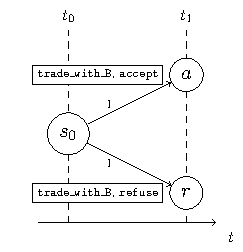
\includegraphics[width=0.4\textwidth]{images/MasterThesisDirectedActionsDraw (2).pdf}
  \end{center}
  \caption{Transition model $\mathcal{T}$ of the trading example. $s_0$ is the initial state, $a$ is the \textit{accept} state, and $r$ is the \textit{refuse} state. The transition model of the environment $\mathcal{T}$ is assumed to be deterministic.}\label{fig:dir1}
\end{figure}





At time $t_0$, agent $A$ performs action \texttt{trade\_with\_B} in state $s_0$. According to \textit{Rens et al.}'s definition of directed actions, the \textit{directed} probability of landing in state $a$ or $r$ at time $t_1$ is conditioned by the reputation of $A$, the agent initiating the trade. 
Consider the following situation: at time $t_0$ agent $A$ has a reputation of $0.5$, which is considered to be relatively good. The probability of $B$ being willing to trade with $A$ is, say, $0.9$, that is,
    \begin{align}
    \label{eq:transitions}
    \begin{split}
        &DT(A, s_0, \texttt{trade\_with\_B}, a, 0.5) = 0.9  \\&  DT(A, s_0, \texttt{trade\_with\_B}, r, 0.5) = 0.1. 
    \end{split}
    \end{align}
Said differently, at time $t_0$, agent $B$ will select action \texttt{accept} with a probability of $0.9$, and action \texttt{refuse} with a probability of $0.1$. 
The problem with the interpretation of the concept of directed actions by \textit{Rens et al.} is twofold:
\begin{itemize}
    \item The first problem resides in the fact that agent $B$ is not aware of agent $A$'s desire to trade at time $t_0$, as agent $A$ has not yet performed \texttt{trade\_with\_B}. Said differently, agent $B$ has no reason to prefer \texttt{accept} over \texttt{refuse} at this point in time.
    \item Suppose now that agent $B$ is made aware of the action agent $A$ is about to perform at $t_0$. The second problem relates to the fundamental properties of transition models. A transition model describes the rules the environment abides by, that is, it explains how the environment reacts \textit{on the basis of the actions taken} by its actors. To move the environment from $s_0$ to $a$, agents $A$ and $B$ need to commit to actions \texttt{trade\_with\_B} and \texttt{accept} respectively. \textit{Directed} transition models fail to be able to describe the rules of the environment. To illustrate the problem clearly, the cases in which $B$ has committed to action \texttt{accept} and in which it has not yet done so will be considered separately: 
    \begin{itemize}
        \item \textbf{Agent $B$ has committed to action \texttt{accept}: }If both agents have committed to their respective actions, then the transitions can simply be explained using \textit{undirected} transitions, that is, transitions that do not depend on the reputation of any agent. As per \RefSec{sub:totaltrans}, the individual \textit{undirected} transitions that explain the rules of the environment as they pertain to agent $A$ are formally given by
        \begin{align*}
            \begin{split}
                UT(A, s_0, \texttt{trade\_with\_B}, a) &= \frac{1}{|\mathcal{A}|} \sum_{a' \in \mathcal{A}} \mathcal{T}(s_0, \texttt{trade\_with\_B}, a', a) 
                \\&= \frac{1}{4} (0 + 1 + 0 + 0) = \frac{1}{4}
                \\&= UT(A, s_0, \texttt{trade\_with\_B}, r)
            \end{split}
        \end{align*}
        
        \item \textbf{Agent $B$ has not yet committed to action \texttt{accept}: }If agent $B$ has not committed to an action yet, then the missing action makes it impossible to use the \textit{transition model of the environment} (\RefSec{sub:totaltrans}) as a basis for deriving the \textit{directed} transition models. Said differently, the directed transitions given in Equation \ref{eq:transitions} can not possibly describe the rules of the environment as they apply to agent $A$. At most, they describe agent $A$'s \textit{subjective} impression of the impact that its own reputation might have on the willingness of agent $B$ to accept its trade offer.
    \end{itemize}
\end{itemize}
A solution to both problems covered in this section will follow in \RefSec{sec:reimagined}.












\subsection{Planning for Optimal Impact}
In RepNet-POMDPs, an agent's ability to thrive in the network is reflected in the reputation it has in the eyes of the remaining agents. A good reputation for agent $g$ increases the likelihood of other agents being willing to \textit{cooperate} with $g$. Moreover, an agent should perform actions according to the \textit{perceived immediate impact} they have on itself.
\begin{definition}[Perceived immediate impact]
\label{def:perceivedpo}
The perceived immediate impact on agent $g$, written $PI_g$, is defined as
    \begin{align*}
        PI_g(B_g,AD_g, a) := &\frac{1}{|\mathcal{G}|} \sum_{s \in \mathcal{S}} b_g^g(s) \big[ \, \mathcal{I}(g,g,s,a) \\&+ \sum_{h \in \mathcal{G} \setminus \{ g \}}  \sum_{a' \in \mathcal{A}} \mathcal{I}(g, h, s, a') b_h^g(s) AD_g(h, s)(a') \, \big]
    \end{align*}
    where
    \begin{itemize}
        \item $a$ is the action performed by agent $g$.
        \item $AD_g$ is the current action distribution of agent $g$.
        \item $B_g$ is the current belief state of agent $g$.
        \item The first term describes the immediate self-impact as a consequence of agent $g$ performing action $a$.
        \item The second describes the expected immediate impact that the network, i.e., the remaining agents, has on agent $g$.
    \end{itemize}
\end{definition}


Analogously to classical POMDPs, a RepNet-POMDP agent $g$ strives to maximize its expected discounted perceived impact
\begin{align}
    \E \big[ \sum_{t = 0}^{k} \gamma^t PI_{g,t}\big]
\end{align}
where $\gamma$ is the \textit{discount factor} and $PI_{g,t}$ is agent $g$'s perceived immediate impact at time-step $t$. This is accomplished by computing the optimal value function $V_g$, as defined in \RefDef{def:optipo}.

\begin{definition} [Value function]
\label{def:optipo}
Let $V_g$ be the optimal value function of agent $g$ in a \textit{finite-horizon} setting. It satisfies the \textit{optimality equations}, which are defined as 
    \begin{align*}
        \begin{dcases}
            V_g(B_g, AD_g, Img_g, k) := &\max_{a \in \mathcal{A}} \Big\{ PI_g(B_g,AD_g,a) \\&+ \gamma \sum_{o \in \Omega} P_g(o | B_g, AD_g, Img_g, a) V_g(B_g', AD_g', Img_g', k-1) \Big\}  
            \\
            V_g(B_g, AD_g, Img_g, 1) := &\max_{a \in \mathcal{A}} \Big\{ PI_g(B_g,AD_g,a) \Big\} 
        \end{dcases}
    \end{align*}
    where
    \begin{itemize}
        \item $B_g' = SE(g, B_g, a, o, Img_g, AD_g)$.
        \item $AD_g' = ADE(g, o, AD_g, Img_g)$.
        \item $Img_g' = IE(g, Img_g, \alpha, B_g, AD_g)$.
        \item $\gamma \in [0,1]$ is called the \textit{discount factor}.
        \end{itemize} 
        
        $P_g(o | B_g, AD_g, Img_g, a)$ can be reformulated using the concepts of observation function, transition model, and belief state (note that the development that follows was left out of Rens et al.'s original paper \cite{rensetal}):
        \begin{align*}
         P_g(o | B_g, AD_g, Img_g, a) &= \sum_{s' \in \mathcal{S}} P_g(o | B_g, AD_g, Img_g, a, s') P_g(s' | B_g, AD_g, Img_g, a)
    \\
    &= \sum_{s' \in \mathcal{S}} P_g(o | a, s') \sum_{s \in \mathcal{S}} P_g(s' | a, s) P_g(s | B_g, AD_g, Img_g, a)
    \\
    &= \sum_{s' \in \mathcal{S}} O_g(g,a, s', o) \sum_{s \in \mathcal{S}} T_g(g, s, a, s',r_g) b_g^g(s)
    \end{align*}



    
\end{definition}
\begin{definition}[Optimal policy]
Let $B_g$ be the current belief state function, $AD_g$ the current action distribution, $Img_g$ the current image function of agent $g$, and $k$ the current horizon. The optimal action for agent $g$, written $\pi(B_g, AD_g, Img_g, k)$, is defined as
\begin{align*}
    \pi(B_g, AD_g, Img_g, k) := &\arg \max_{a \in \mathcal{A}} \Big\{ PI_g(B_g,AD_g,a) \\&+ \gamma \sum_{o \in \Omega} P_g(o | B_g, AD_g, Img_g, a) V_g(B_g', AD_g', Img_g', k-1) \Big\}.
\end{align*}
\end{definition}
